\documentclass	[11pt, a4paper, openany]{book}
\usepackage{Preambule}
\usepackage[T1]{fontenc}
\usepackage{mathpazo}
\usepackage[scaled=0.95]{helvet}
\usepackage{courier}
\usepackage{caption}
\usepackage{adjustbox}
\usepackage{listings}
\usepackage{color} %red, green, blue, yellow, cyan, magenta, black, white
\definecolor{mygreen}{RGB}{28,172,0} % color values Red, Green, Blue
\definecolor{mylilas}{RGB}{170,55,241}
\newcommand{\HRule}{\rule{\linewidth}{0.5mm}}
\renewcommand*{\figureautorefname}{Fig.}
\usepackage[style=alphabetic,backend=biber,url=true,natbib=true]{biblatex}
\DeclareFieldFormat{url}{\space\url{#1}}
\DeclareNameAlias{default}{last-first}
\renewcommand\nameyeardelim{, }
\addbibresource{a.bib}
\usepackage[autostyle]{csquotes}

\newcommand{\prop}[1]{\adjustbox{minipage=\linewidth-2\fboxsep-2\fboxrule,fbox}{
#1}}

\begin{document}
\AddToShipoutPicture*{\BackgroundPic}
\begin{titlepage}
\begin{center}	
	
	\newcommand{\HRule}{\rule{\linewidth}{0.5mm}}   			            %Titre en gros
	
\includegraphics[scale=0.11]{titlepage/logo.jpg}~\\[1cm]				%Logo

	\textsc{\LARGE Université Libre de Bruxelles}\\[1.5cm]
	\textsc{\Large Synthèse}\\[0.5cm]

	\HRule \\[0.4cm]
	{ \huge \bfseries Mécanique du solide et résistance des matériaux \ \\CNST-H-2001 \\[0.4cm] }


	\HRule \\[1.5cm]
		\begin{minipage}{0.4\textwidth}
		\begin{flushleft} \large
		
		\emph{Auteur :}\\
			Nicolas \textsc{Englebert}

			\end{flushleft}
			\end{minipage}
			\begin{minipage}{0.4\textwidth}
			\begin{flushright} \large
			%\emph{Tuteur :} \\		
			\end{flushright}
		\end{minipage}

	\vfill

% Bottom of the page
{\large Année 2015 - 2016}

\end{center}
\end{titlepage}


\tableofcontents

\chapter{Les circuits réactifs en régime - Phaseurs et impédances}

\section{Partie pratique}
\subsection{Question 1}
\begin{center}
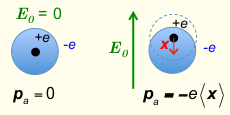
\includegraphics[scale=0.7]{image1.png}
\captionof{figure}{\label{fig:01}Schéma de la question 1}
\end{center}

\subsubsection{Sous-question a}
\prop{Régler le générateur de fonction selon les paramètres de la TABLE 1.1. Mesurer la
tension à vide à l’aide du multimètre.\\
Brancher ensuite le générateur à l’oscilloscope. Sans utiliser l’AUTO SET, régler l’oscilloscope
de manière à pouvoir observer 2 périodes. Quels paramètres ont dus être modifiés
? Mesurer la tension et la période du signal à l'aide de l'oscilloscope.}\ \\

Premièrement il nous a fallu régler le générateur de tension qui était initialement réglé sur \textit{peak to peak} pour le faire considérer des \textit{valeurs efficaces}. \\
En appuyant sur la valeur $4\ V$, nous avons ensuite choisi $V_{RMS}$. La fréquence a ensuite été réglée grâce au bouton \textit{Freq}  sur $20\ kHz$.\\

Le générateur de tension étant réglé, nous avons pu mesurer la tension à vide avec le multimètre. Nous avons réglé celui-ci en tension alternative puis connecté au générateur de tension.
\begin{equation}
V_{vide} = 4,028\ V
\end{equation}

Nous avons ensuite branché le générateur de tension à l'oscilloscope à l'aide des adaptateurs \textit{BNC-Bananes}. Les masses de ces deux appareils étant identiques, nous avons pris soin de les connecter entre elles.\\
Afin d'obtenir deux périodes, nous avons dû apporter des modifications aux molettes suivante :
\begin{itemize}
\item L'échelle verticale ($V/div$)
\item Le positionnement vertical
\item L'échelle horizontale ($s/div$)
\item Le positionnement horizontal
\end{itemize}
L'oscilloscope nous donnait directement accès aux mesures de la période et de la tension (peak to peak et efficace).
\begin{eqnarray}
V_{pp} &=& 11.1\pm 0.1\ V\\
V_{RMS} &=& 4.13\ V\\
T &=& 50.00\pm 0.01\ \mu s
\end{eqnarray}

\subsubsection{Sous-question b}
\prop{Réaliser le montage ci-dessus en utilisant les paramètres de la TABLE 1.1.}\ \\
Nous avons ensuite réalisé le montage présenté ci-dessus (\autoref{fig:01}).\footnote{Photo Benoît}

\subsubsection{Sous-question c}
\prop{Vérifier la loi des mailles de ce circuit en utilisant les phaseurs (algébriquement et
graphiquement).\\
Proposer un plan de travail détaillé utilisé pour répondre à la question (ex : mesures à
réaliser, points d'attention, etc)
Aide:\\
— Commencer par prendre une mesure de la différence de potentiel aux bornes de
chacun des composants du circuit et utiliser-les comme point de départ\\
Consignes :\\
— Exprimer les amplitudes des grandeurs en valeurs efficaces ($V_{eff}$) et les décalages
temporels en degré}\ \\
Il faut commencer par mesurer la tension aux bornes de chaque composant. L'amplitude de chaque signal donne la norme du phaseur tandis que le déphasage s'obtient en mesurant le décalage temporel avec le signal du générateur sur l'oscilloscope. Chaque phaseur peut alors s'écrire sous la forme d'une partie réelle et d'une partie imaginaire. La somme des parties réelles,respectivement imaginaires, des phaseurs des tensions mesurées sera égale à la partie réelle,respectivement imaginaire, du phaseur de la tension du générateur.\\

Afin de mesurer les tensions de chaque élément du circuit ainsi que leurs déphasages nous avons choisi de prendre le courant comme référence. Nous pouvons effectivement l'obtenir de façon simple grâce à la présence de la résistance dans notre montage. Nous savons qu'il n'y a pas de déphasage entre courant et tension au niveau de la résistance.\\
\begin{center}
\begin{tabular}{|c|c|c|}
\hline 
\textbf{Composant} & \textbf{Tension} ($V_{RMS}$) & \textbf{Déphasage} ($s$) \\ 
\hline 
$R_e$ & $1.00$ & 0 \\ 
\hline 
$Z_j$ & $245*10^{-3} \pm 5*10^{-3}$ & 0 \\ 
\hline 
$Z_i$ & $150*10^{-3}\pm 5*10^{-3}$ & $12.00*10^{-6}$ \\ 
\hline 
Générateur & $1.32$ & $4.78*10^{-6}$ \\ 
\hline 
\end{tabular} 
\end{center}
Pour calculer la tension aux bornes de $Z_j$ nous avons effectué la différence entre la tension aux bornes de $R_e +Z_j$ et celle aux bornes de $R_e$. De façon analogue la tension aux bornes de $Z_i$ se calcule en effectuant la différence entre la tension aux bornes du générateur par la tension aux bornes de $R_e + Z_j$. Pour la tension aux bornes de $R_e$, nous l'avons calculée de façon directe.\\

Étant donné que nous avons calculé les différences de tension à l'aide de l'oscilloscope nous avons pu mesurer graphiquement (et précisément avec les curseurs) le déphasage temporel entre nos tensions en prenant pour référence la tension aux bornes de $R_e$ (car son déphasage avec le courant est nul, c'est donc équivalent à prendre le courant comme référence).
 

Pour convertir le déphasage mesuré en seconde en radian, nous devons utiliser les transformations suivantes :
\begin{equation}
\sin(\omega t + \phi) \Leftrightarrow \sin(\omega(t+\frac{\phi}{\omega}))
\end{equation}
Nous savons que $\frac{\phi}{\omega}$ correspond à notre déphasage temporel, ce qui nous permet de retrouver le déphasage en radian
\begin{equation}
\Delta t = \frac{\phi}{\omega} \Leftrightarrow \phi = \omega*\Delta t
\end{equation}
Avec les données expérimentales, nous retrouvons les déphasages suivants :
\begin{eqnarray}
\phi_{Z_i} = 86.4 \deg\\
\phi_{gen} = 34.4 \deg
\end{eqnarray}

Vérifions dès à présent la loi des mailles en phaseurs. Écrivons d'abord la loi des mailles :
\begin{equation}
V_{AC} e^{i\theta_{AC}} = V_{i} e^{i\theta_{i}} + V_{j} e^{i\theta_{j}} + V_{e} e^{i\theta_{e}}
\end{equation}
En considérant les parties réelles et imaginaires, nous obtenons :
\begin{equation}
\left\{\begin{array}{l}
V_{AC}\cos(\theta_{AC}) = V_i\cos(\theta_i) + V_j\cos(\theta_j) + V_e\cos(\theta_e)\\
V_{AC}\sin(\theta_{AC}) = V_i\sin(\theta_i) + V_j\sin(\theta_j) + V_e\sin(\theta_e)
\end{array}\right.
\end{equation}
En remplaçant chacune des inconnues par sa valeur mesurée expérimentalement, nous observons bien une vérification de la loi des mailles.

\subsubsection{Sous-question d}
\prop{Caractériser les 3 impédances composant le circuit.}\ \\

Afin de caractériser les différentes impédances, nous avons besoin de déterminer le courant. 
\begin{equation}
I_{eff} = \dfrac{V_{R_e}}{R_e} = \dfrac{1.00\ V}{20\ \Omega} = 50.0\ mA
\end{equation}
La valeur de la résistance ainsi que celle du courant ont été confirmées grâce aux mesures obtenues à l'aide du multimédia.\\

Les données expérimentales montrent que la tension est en avance sur le courant pour $Z_i$, ce qui nous permet de conclure que ce composant est une self. N'ayant aucun déphasage pour $Z_j$, nous en concluons qu'il s'agit d'une résistance.\\
Les impédances des différents composantes sont les suivantes :
\begin{eqnarray}
Z_{R_e} &=& \dfrac{V_{R_e}}{I_{eff}} = 20\ \Omega\\
|Z_i| &=& \dfrac{V_{Z_i}}{I_{eff}} = 3.02\ \Omega\\
|Z_j| &=& \dfrac{V_{Z_j}}{I_{eff}} = 4.71 \Omega
\end{eqnarray}
A partir de ces impédances, calculons les valeurs réelles de ces composants :
\begin{eqnarray}
|Z_i| = \omega L_i \Leftrightarrow L_i = \dfrac{|Z_i|}{\omega} = 22.9\ \mu H\\
R_i = |Z_j| = 4.71\ \Omega
\end{eqnarray}








\newpage
\subsection{Question 2}
\begin{center}
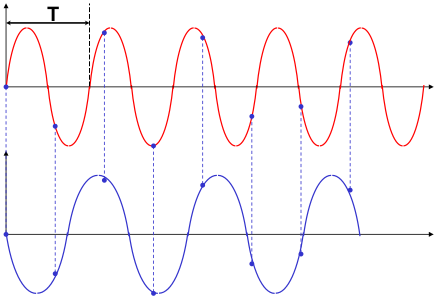
\includegraphics[scale=0.7]{image2.png}
\captionof{figure}{\label{fig:02}Schéma de la question 2}
\end{center}
\subsubsection{Sous-question a}
\prop{Réaliser le montage ci-dessus en utilisant les $Z_i$ et $Z_j$ de votre montage précédent
ainsi que les paramètres définis dans la TABLE 1.2.}\ \\
Nous avons réalisé le montage présenté ci-dessus (\autoref{fig:02}).


\subsubsection{Sous-question b}
\prop{Connaissant la valeur de tous les paramètres,\\
— Prédire par calculs la différence de potentiel (ddp) aux bornes de chacun des
composants\\
— Vérifier ensuite ces valeurs expérimentalement}\ \\

Commençons par écrire les équations de notre circuit
\begin{equation}
\left\{\begin{array}{l}
\underline{V_{AC}} = (Z_1 + Z_2 + R_e + R_g)\underline{I} - Z_2\underline{I_2}\\
Z_2\underline{I_1} = Z_3\underline{I_2}\\
\underline{I} = \underline{I_1} +\underline{I_2}
\end{array}\right.
\end{equation}
Résolvons ce système :
\begin{equation}
\left\{\begin{array}{l}
\underline{V_{AC}} = (Z_1 + Z_2 + R_e + R_g)\underline{I_1} + (Z_1 + R_e + R_g)\underline{I_2}\\
\underline{I_2} = \dfrac{Z_2}{Z_3}\underline{I_1}\\
\underline{I} = \underline{I_1} +\underline{I_2}
\end{array}\right.
\end{equation}
En remplaçant la deuxième ligne dans la première équation :
\begin{equation}
\left\{\begin{array}{l}
\underline{V_{AC}} = (Z_1 +Z_2 +R_e + R_g)\underline{I_1} + (Z_1 + R_e + R_g)\dfrac{Z_2}{Z_3}\underline{I_1}\\
\underline{I_2} = \dfrac{Z_2}{Z_3}\underline{I_1}\\
\underline{I} = \underline{I_1} +\underline{I_2}
\end{array}\right.
\end{equation}
Le système est résolu :
\begin{equation}
\left\{\begin{array}{l}
\underline{I_1} = \dfrac{\underline{V_{AC}}}{Z_1 + Z_2 + R_e + R_g + \frac{Z_1Z_2}{Z_3} + \frac{R_eZ_2}{Z_3} + \frac{R_gZ_2}{Z_3}}\\
\underline{I_2} = \dfrac{Z_2}{Z_3}\underline{I_1}\\
\underline{I} = \underline{I_1} +\underline{I_2}
\end{array}\right.
\end{equation}
Grâce aux données de l'exercice précédents, nous pouvons calculer les courants théoriques : 
\begin{equation}
\left\{\begin{array}{l}
\underline{I_1} = 0.05343 - 0.0277i\\
\underline{I_2} = 0.014427 + 0.02783i\\
\underline{I} = 0.06786 + 1,2874*10^{-4}i
\end{array}\right.
\end{equation}
Nous pouvons en profiter pour calculer les valeurs réelles de ces courants : 
\begin{equation}
\left\{\begin{array}{l}
I_1 = 59\ mA\ \ \ \ \ \ \ (\text{Résultat mesuré : 55.0 mA})\\
I_2 = 31.3\ mA\ \ \ \ (\text{Résultat mesuré : 29.7 mA})\\
I = 67.8\ mA\ \ \ \ \ \ (\text{Résultat mesuré : 61.8 mA})
\end{array}\right.
\end{equation}

Ces résultats nous permettent de calculer les différentes tensions de notre circuit:
\begin{equation}
\left\{\begin{array}{l}
V_g\ \  = 1.607\ V\\
V_{Z_1} = 0.750\ V\\
V_{Z_2} = 0.283\ V\\
V_{R_e} = 1.357\ V
\end{array}\right.
\end{equation}



Pour vérifier ces valeurs, nous avons relevé les tension de chacun des composants expérimentalement :
\begin{equation}
\left\{\begin{array}{l}
V_g\ \  = 1.765\ V\\
V_{Z_1} = 0.756\ V\\
V_{Z_2} = 0.273\ V\\
V_{R_e} = 1.319\ V
\end{array}\right.
\end{equation}







\newpage
\subsection{Question 3 - BONUS}
\begin{center}
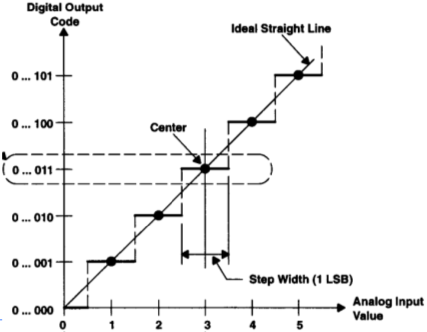
\includegraphics[scale=0.7]{image3.png}
\captionof{figure}{Schéma de la question 3}
\end{center}
\subsubsection{Sous-question a}
\prop{Associez-vous avec un autre groupe et réalisez le montage ci-dessous. Gardez les
impédances $Z_i$ et $Z_k$ d’un seul des deux groupes. Paramétrez les deux générateurs de
fonction sinusoïdale à des fréquences différentes.}\


\subsubsection{Sous-question b}
\prop{Afin de résoudre ce circuit, quel nouveau principe/méthode devez-vous utilisez ?}\ \\
Le principe de superposition permettra de résoudre ce circuit. Ce principe énonce que la réponse d'un système à la somme de deux signaux est la même que la somme des réponses du circuit aux deux signaux séparément.


\subsubsection{Sous-question b'}
\prop{Ce principe aurait-il pu être utiliser si les deux générateurs étaient mis en série.}\ \\
Non, car les mettre en série aurait causé un problème avec les masses : un des générateurs auraient été court-circuité.

\subsubsection{Sous-question c}
\prop{Vérifier la loi des mailles de ce circuit en utilisant les phaseurs (algébriquement et
graphiquement).\\
Proposer un plan de travail détaillé utilisé pour répondre à la question (ex : mesures à
réaliser, points d'attention, etc).}\


Commençons par écrire les équations de ce circuit : 
\begin{equation}
\left\{\begin{array}{l}
\underline{V_1} = Z_i\underline{I_1} + Z_k\underline{I_1} + R_1\underline{I_1}\\
\underline{V_2} = Z_k \underline{I_2} + R_2\underline{I_2}\\
\underline{V_2} = Z_i \underline{I_3} + R_2\underline{I_2}
\end{array}\right.
\end{equation}
En isolant les courants :
\begin{equation}
\left\{\begin{array}{l}
\underline{I_1} = \dfrac{\underline{V_1}}{Z_i + Z_k + R_1}\\
\underline{I_2} = \dfrac{\underline{V_2}}{Z_k + R_2}\\
\underline{I_3} = \dfrac{\underline{V_2}}{Z_i + R_2}
\end{array}\right.
\end{equation}
Nous obtenons ainsi les tension aux bornes des deux composantes\footnote{$R_1$ et $R_2$ sont les résistances internes respectivement du générateur 1 et 2.} :
\begin{equation}
\left\{\begin{array}{l}
\underline{V_i}(e^{i\omega_1t}+e^{i\omega_2t}) = Z_i(\underline{I_1}e^{i\omega_1t} - \underline{I_3}e^{i\omega_2t}) = Z_i\left(\dfrac{\underline{V_1}}{Z_i+Z_k + R_1}e^{i\omega_1t}-\dfrac{\underline{V_2}}{Z_i + R_2}e^{i\omega_2t}\right)\\
\underline{V_k}(e^{i\omega_1t}+e^{i\omega_2t}) = Z_i(\underline{I_1}e^{i\omega_1t} + \underline{I_2}e^{i\omega_2t}) = Z_k\left(\dfrac{\underline{V_1}}{Z_i+Z_k + R_1}e^{i\omega_1t}+\dfrac{\underline{V_2}}{Z_k + R_2}e^{i\omega_2t}\right)
\end{array}\right.
\end{equation}
Ceci n'est pas faisable en phaseurs, mais en passant dans le domaine temporel nous pouvons solutionner ces équations.
















\chapter{Les circuits réactifs en transitoire}
\section{Partie pratique}
\subsection{Visualisation d'un phénomène périodique lent [20 min]}
\textit{Appliquer au canal 1 ($CH1$) l’oscilloscope un signal triangulaire produit par un générateur de
fonction. Ce signal doit avoir une fréquence $f$ = 1 $Hz$ et une amplitude crête-à-crête d’environ
1, 5V}
\subsubsection{Sous-question a}
\prop{Il est demandé de faire une acquisition à l’oscilloscope de ce signal sur deux période
(image non défilante).\\
Détailler ci-dessous la démarche utilisé.\\
— Si des fonctions de l’oscilloscope sont utilisées, noter leurs noms et expliquer
brièvement quel est leur utilité.\\
— Si des paramètres de réglage de l’oscilloscope doivent être modifiés, noter leurs
noms et les valeurs choisies.}\ \\
Nous avons premièrement commencé à effectuer les réglages préliminaires, à savoir produire un signal triangulaire d'une fréquence de 1 Hz, et d'une amplitude \textit{peak-to-peak} de 1.5 V.\\
Les deux seules fonctions utilisées sont celles permettant de placer notre signal aux zéros de nos deux axes, respectivement la tension et le temps.\\

En ce qui concerne les paramètres, nous avons choisi comme échelle verticale \textit{200 mV/div} et comme échelle horizontale \textit{200ms/div}. Le \textit{trigger} a été réglé de façon automatique pour empêcher tout défilement.


\subsubsection{Sous-question b}
\textit{Réaliser un déclenchement sur pente montante avec le menu TRIGGER. Placez d’abord, votre
niveau de déclenchement ainsi que votre niveau de base du signal à $0V$. Placez également le
moment de déclenchement au centre de l’écran (à 0s).}\\
\prop{Noter votre choix de réglage pour chaque paramètre du menu TRIGGER. Expliquer}\ \\

En accédant au menu du TRIGGER, type \textit{SLOPE}, nous réglons ensuite le paramètre \textit{WHEN} sur la pente montante.\\



\subsubsection{Sous-question c}
\prop{Que se passe-t-il lorsque vous\\
— modifiez le niveau de déclenchement ?\\
— modifiez le niveau de base ?\\
— choisissez une pente descendante pour le déclenchement ?\\
Expliquez.}\ \\

Lorsque nous déplaçons le niveau de déclenchement, nous observons une translation horizontale de la courbe. Ceci est dû à la modification du point d'intersection du trigger avec l'axe vertical et donc de l'intersection de la courbe avec l'axe vertical.\\

Si l'on place le niveau de déclenchement au dessus de notre courbe, l'oscilloscope se place en mode \textit{WAIT}. Comme le TRIGGER n'intercepte pas la courbe, elle ne peut simplement pas s'actualiser.\\ 
Lorsque le voltage atteint le niveau de déclenchement, le signal est centré sur l'ordonnée.

La modification de niveau de base permet simplement une translation
verticale de notre signal.\\

Les conclusions tirée pour la pente montante sont les mêmes que pour un pente descendantes.




\newpage
\subsection{Étude d’un phénomène transitoire (source de tension continue) [80min]}
\textit{Réaliser le montage de la figure ci-dessous.}
\begin{center}
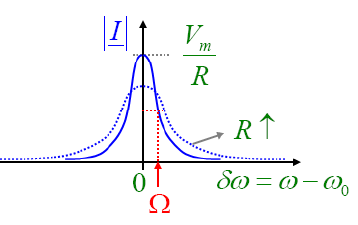
\includegraphics[scale=0.7]{image21.png}
\captionof{figure}{\label{fig:21}Schéma de la question 1}
\end{center}

\textit{Avec :}
\begin{itemize}
\item $V_S$ : source de tension continue (environ $5V$)
\item $R_e$ : résistance étalon ($20\Omega$)
\item $T_0$ : interrupteur
\item $L, R_L$ : inductance
\end{itemize}

\subsubsection{Sous-question a}
\prop{Déterminer analytiquement l’évolution du courant dans ce circuit pour tout temps $t$
si on ferme l’interrupteur en $t = 0s$.}\ \\

Avant la fermeture de l'interrupteur, le courant est nul car le circuit est ouvert. Nous avons donc que $I(t) = 0\, \forall t < 0$. En particulier, $I(0^-) = 0$.

Pour résoudre ce circuit une fois l'interrupteur fermé, commençons par écrire la loi des mailles : 
\begin{equation}
 V_S = L \dfrac{dI}{dt} + RI
\end{equation}
où $R = R_L + R_e + R_g$
Afin de résoudre cette équation différentielle, commençons par écrire l'équation homogène :
\begin{equation}
 L \dfrac{dI}{dt} + RI = 0
\end{equation}

Il s'agit d'une équation différentielle à variables séparées, dont la solution est de la forme :
\begin{equation}
I(t) = A e^ {- \frac{R}{L} t}
\end{equation}

À cela il faut rajouter la solution particulière, qui ici est une constante\footnote{La tension étant constante} :
\begin{equation}
I(t) = A e^ {- \frac{R}{L} t} + B
\end{equation}

Par continuité du courant à travers l'inductance, nous savons que $I(0^+) = I(0^-) = 0$. Nous en déduisons que $A = -B$ et nous pouvons donc réécrire le courant sous la forme :
\begin{equation}
I(t) = A (e^ {- \frac{R}{L} t}-1)
\end{equation}

De plus, le courant étant nul à l'instant $t=0^+$, la ddp aux bornes des résistance l'est aussi et la loi des mailles s'écrit donc :
\begin{equation}
V_S = - RA e^ {- \frac{R}{L} 0} = -RA
\end{equation}

Nous trouvons donc la valeur de $A$ :
\begin{equation}
A = -\frac{V_S}{R}
\end{equation}

Et donc l'expression du courant $\forall t > 0$ :
\begin{equation}
I(t) = \dfrac{V_S}{R} \left(1 - e^ {- \frac{R}{L} t}\right)
\end{equation}

Le courant pour tout temps $t$ est donc donné par :
\begin{equation}
I(t) = \left\{\begin{array}{ll}
0 & t<0 \\
\dfrac{V_S}{R} \left(1 - e^ {- \frac{R}{L} t}\right) &  t\geq 0
\end{array}\right.\end{equation}

\subsubsection{Sous-question b}
\prop{Que représente le paramètre $R_L$ ?}\ \\
Le paramètre  $R_L$ représente la résistance interne de l'inducteur. En effet, il ne s'agit pas d'un inducteur idéal mais bien un inducteur réel ce qui implique que son impédance n'est pas purement imaginaire mais comporte aussi une partie réelle. Celle-ci est modélisée par une résistance et représente le fait que le courant sera en partie dissipé par effet Joule à l'intérieur des fils de l'inductance.

\subsubsection{Sous-question c}
\prop{On désire mesurer la tension aux bornes de l’inductance à l’aide de l’oscilloscope.
Comment allez-vous procéder ? Ajouter sur le schéma ci-dessus le(s) point(s) de mesure(
s) à l’oscilloscope et expliquer.}\ \\

Il est important de ne pas créer de court-circuit en mesurant la tension sur nos composants. Pour cela, il faut obligatoirement relier les masses du circuit et de l'oscilloscope entre elles. Comme nous avons un montage en série, l'ordre des composants n'a pas d'importance, et nous pouvons donc relier une des deux bornes de l'inductance réelle (donc les composants $R_L$ et $L$) à la masse, et brancher la sonde de l'oscilloscope à ses bornes.

\begin{center}
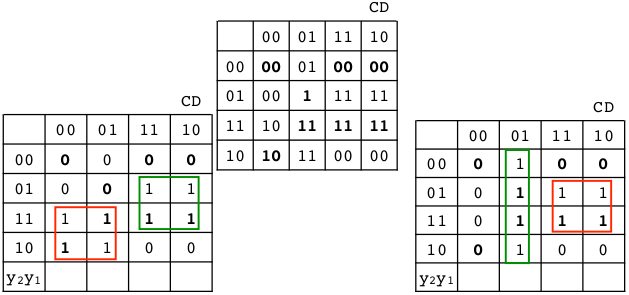
\includegraphics[scale=0.6]{image23.png}
\captionof{figure}{\label{fig:23}Points de prise de tension, question 1.2.1 c}
\end{center}


\subsubsection{Sous-question d}
\textit{Il est demandé de faire une analyse du transitoire de ce circuit lorsque l’interrupteur est appuyé. Configurer donc l’oscilloscope et utilisez la fonction TRIGGER.}\\
\prop{Quelles doivent être les valeurs des paramètres de l’oscilloscope que afin d’observer le
transitoire ? En particulier, le niveau, le moment et la source de déclenchement.}\ \\

Le niveau de déclenchement est de $4\ V$ (nous espérons un échelon de 5 $V$). Le moment de déclenchement est de $40\ ms$.\\
Nous avons ensuite réglé la source de déclenchement sur une pente montante du $CH1$.\\
L'échelle de temps a été prédéfinie à $10\ ms/div$ et celle de tension à $1.00\ V/div$ avec un OFFSET de $-2.00\ V$.\\
Nous obtenons bien une exponentielle décroissante comme nous l'avions prévu. En effet, le courant étant initialement nul, toute la tension doit se retrouver en intégralité aux bornes de notre self. La tension doit ensuite décroitre pour devenir nulle aux bornes de la self en situation de régime. Comme $R_L$ était compris dans notre mesure, la tension de régime mesurée n'est pas nulle mais vaudra :
\begin{equation}
V_{R_L} = \dfrac{R_L}{R_e + R_L}V_s
\end{equation}

\subsubsection{Sous-question e}
\textit{Une fois la paramétrisation effectuée, armer l’oscilloscope et fermer l’interrupteur.}\\

\prop{Déterminer à partir des résultats obtenus à l’oscilloscope, la constante de temps $\tau$ du
circuit réalisé ainsi que la valeur de régime du courant dans le circuit. Expliquer à l’aide
d’un graphe.\\
— Pour les calculs, se baser sur l’exercice préliminaire et sur la question a)\\
— Utiliser les curseurs}\ \\
La constante de temps $\tau$ obéit à la relation suivante :
\begin{equation}
 \tau = \frac{L}{R} 
\end{equation}
Celle-ci est caractérise l'ordre de grandeur du temps au bout duquel le nouvel équilibre est atteint. On sait que la sortie atteint 95\% de sa valeur en régime à $3\tau$ et 99.3\% après $5\tau$ (et 63\% après $\tau$).\\

%\begin{center}
%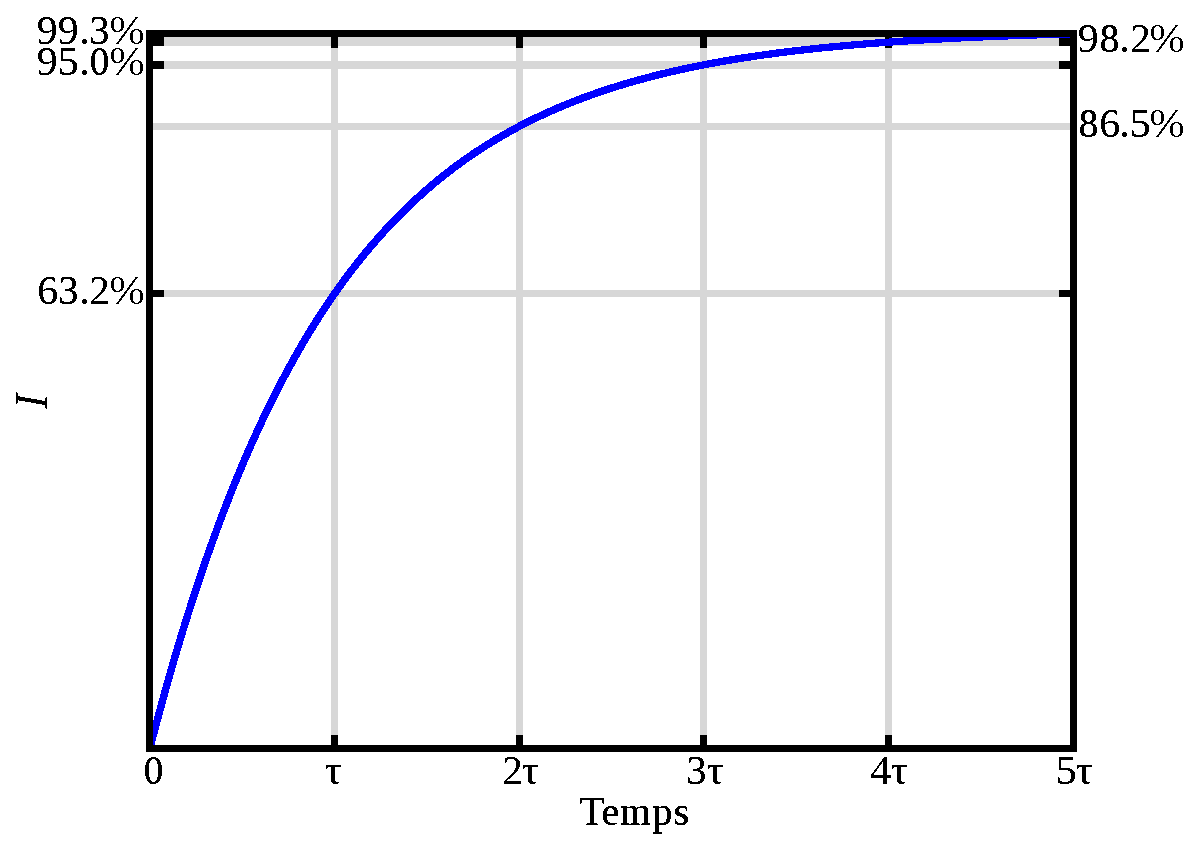
\includegraphics[scale=0.3]{image24.pdf}
%\captionof{figure}{\label{fig:24}Évolution vers le régime stationnaire (jusqu'à 5$\tau$)}
%\end{center}

Nous avons mesuré que la tension en régime est de $3.3\ V$ ce qui correspond à une chute de tension de $1.7\ V$. Après un temps $\tau$, 63\% de la décharge est effectuée, il reste donc 37\% de la tension initialement présente (1.7 $V$). 
\begin{equation}
37\% * 1.7V + 3.3 V = 3.92\ V
\end{equation}
Le temps après lequel la tension est de 3.92 $V$ est de :
\begin{equation}
\tau = 21.4\ ms
\end{equation}



\subsubsection{Sous-question f}
\prop{Déterminer les valeurs de la tension aux bornes de l’inductance en régime $V_{ind_{regime}}$,
de la résistance $R_L$ et de l’inductance $L$.}\ \\

La loi basse-fréquence de l'inducteur idéal stipule que la tension aux bornes de l'inducteur est nulle après un temps suffisamment long à cause de la loi $V_L = L.\frac{d}{dt}i(t)$. L'inducteur réel est ici modélisé par un inducteur fictif mis en série avec une résistance. La chute de potentiel aux bornes de l'inducteur fictif sera nulle à cause de la loi basse fréquence. La différence de potentiel aux bornes de l'inducteur du circuit sera donc égale à la chute de potentiel due à la partie résistive de l'inducteur. On aura donc $V_{ind_{regime}} = R_L.i(t)$.\\

Nous commençons par mesurer la tension en régime : 
\begin{equation}
V_{ind_{regime}} = 3.3\ V
\end{equation}
En régime, nous savons que $V_L = 0\ V$ et la loi des mailles peut donc s'écrire :
\begin{equation}
V_s = (R_e + R_L)I
\end{equation}
La tension aux bornes de $R_L$ est donc donnée par :
\begin{equation}
V_{R_L} = \dfrac{R_L}{R_e + R_L}V_s
\end{equation}
En remplaçant par les valeurs, nous obtenons :
\begin{equation}
3.3\ V = \dfrac{R_L}{20\ \Omega + R_L}5\ V
\end{equation}
Ce qui donne :
\begin{equation}
R_L = 38.8\ \Omega
\end{equation}
En partant de l'expression de $\tau$, on obtient :
\begin{equation}
L = \tau(R_e + R_L)
\end{equation}
Ce qui nous donne:
\begin{equation}
L = 1.26\ H
\end{equation}




\newpage
\subsection{Courant transitoire dans une inductance (source de tension sinusoïdale) [100min]}
\begin{center}
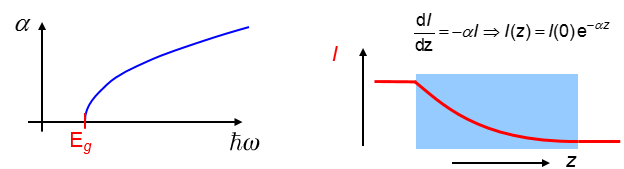
\includegraphics[scale=0.7]{image22.png}
\captionof{figure}{\label{fig:22}Schéma de la question 2}
\end{center}
\textit{Réaliser le montage de la figure ci dessus, avec :}
\begin{itemize}
\item $T_0$ : interrupteur
\item $V_S(t)$ : source de tension d'amplitude $6V$ (\textit{peak-to-peak}) et de fréquence 50 $Hz$ provenant du générateur de fonctions
\item $L$ : inductance à noyau de fer
\item $R_e$ : résistance étalon (20 $\Omega$)
\end{itemize}

\subsubsection{Sous-question a}
\prop{Quelle est la principale différence entre ce circuit et le précédent ?}\ \\
Le circuit est soumis à une excitation de type sinusoïdale.


\subsubsection{Sous-question b}
\prop{Déterminer analytiquement l’évolution du courant dans ce circuit pour tout temps t
si l’interrupteur est fermé en $t = 0$.}\ \\

Avant la fermeture de l'interrupteur, le courant est nul car le circuit est ouvert. Nous avons donc que $I(t) = 0\, \forall t < 0$. En particulier, $I(0^-) = 0$.

Pour résoudre ce circuit une fois l'interrupteur fermé, commençons par écrire la loi des mailles : 
\begin{equation}
 V_S = L \dfrac{dI}{dt} + RI
\end{equation}
où $R = R_L + R_e + R_g$. Afin de résoudre cette équation différentielle, commençons par écrire l'équation homogène :
\begin{equation}
 L \dfrac{dI}{dt} + RI = 0
\end{equation}

Il s'agit d'une équation différentielle à variables séparées, dont la solution est de la forme :
\begin{equation}
I(t) = A e^ {- \dfrac{R}{L} t}
\end{equation}

À cela il faut rajouter la solution particulière. Notre terme non-homogène étant de forme sinusoïdale\footnote{$V_m\cos(\omega t + \alpha)$},
la solution particulière sera de la forme :
\begin{equation}
i_{SPENH}(t) = B\cos(\omega t + \alpha) + C\sin(\omega t + \alpha)
\end{equation}
En substituant cette équation dans l'équation du circuit, on trouve : 
\begin{equation}
R[B\cos(\omega t + \alpha) + C\sin(\omega t + \alpha)] + L[-\omega B\sin(\omega t + \alpha)+\omega\cos(\omega t + \alpha)] = V_m\cos(\omega t + \alpha)
\end{equation}
Par identification :
\begin{equation}
\left\{\begin{array}{ll}
 RB + \omega LC & = V_m  \\
 -\omega LB + RC & = 0 
\end{array}\right.
\end{equation}
Les coefficients indéterminés valent ainsi :
\begin{equation}
\left\{\begin{array}{ll}
 B = & \frac{RV_m}{R^2 + (\omega L)^2}  \\
 C = &  \frac{\omega LV_m}{R^2 + (\omega L)^2}
\end{array}\right.
\end{equation}
Notre solution particulière est :
\begin{equation}
i_{SPENH}(t) = \frac{RV_m}{R^2 + (\omega L)^2}\cos(\omega t + \alpha) +  \frac{\omega LV_m}{R^2 + (\omega L)^2}\sin(\omega t + \alpha)
\end{equation}

La solution générale est alors :
\begin{equation}
i(t) = A e^ {- \dfrac{R}{L} t} + \frac{RV_m}{R^2 + (\omega L)^2}\cos(\omega t + \alpha) +  \frac{\omega LV_m}{R^2 + (\omega L)^2}\sin(\omega t + \alpha)
\end{equation}

Il nous faut maintenant déterminer la constante $A$ grâce à la condition initiale $i(t_0^-) = i(t_0^+) = 0$. En en tire :
\begin{equation}
i(t_0^+) = Ae^0 + \frac{RV_m}{R^2 + (\omega L)^2}\cos(\omega 0 + \alpha) +  \frac{\omega LV_m}{R^2 + (\omega L)^2}\sin(\omega 0 + \alpha) = 0
\end{equation}
\begin{equation}
\Rightarrow A = -\left(\frac{RV_m}{R^2 + (\omega L)^2}\cos(\alpha) +  \frac{\omega LV_m}{R^2 + (\omega L)^2}\sin(\alpha)\right)
\end{equation}

Le courant s'exprime donc sous la forme :
\begin{equation}
i(t) = -\left(\frac{RV_m}{R^2 + (\omega L)^2}\cos(\alpha) +  \frac{\omega LV_m}{R^2 + (\omega L)^2}\sin(\alpha)\right) e^ {- \frac{R}{L} t} + \frac{RV_m}{R^2 + (\omega L)^2}\cos(\omega t + \alpha) +  \frac{\omega LV_m}{R^2 + (\omega L)^2}\sin(\omega t + \alpha)
\end{equation}

\subsubsection{Sous-question c}
\textit{On vous demande de faire une analyse des transitoires possibles des tensions aux bornes de la
résistance et de l’inductance de ce circuit lorsque l'interrupteur $T_0$ est appuyé. Configurer donc
l’oscilloscope et utiliser la fonction TRIGGER.}\\

\prop{Quelles sont les valeurs des paramètres de l’oscilloscope que vous avez utilisé pour observer
le transitoire ? En particulier, la source, le niveau et le moment de déclenchement
ainsi que les bases de temps et de tension.}\ \\

Nous avons mis la source sur le $CH1$, le niveau de déclenchement à $50\ mV$, le moment de déclenchement à $40\ ms$, la base de temps à $10\ ms/div$, la base de tension aux bornes de la résistance à $100\ mv/div$ et celle aux bornes du générateur à $1.00\ V/div$.


\subsubsection{Sous-question d}
\textit{Fermer quelques fois l’interrupteur $T_0$. Conserver une acquisition avec un transitoire important et une acquisition avec un transitoire quasi inexistant.}\\
\prop{Dans chaque cas, déterminer sur base des résultats obtenus à l’oscilloscope :\\
— le facteur de surintensité de courant $F = \frac{\text{1ere crête}}{\text{1ere crete (regime)}}$\\
— l’écart temporel Dt entre l’instant de fermeture de l’interrupteur et l’instant de
passage à zéro montant de la tension appliquée $v_S(t)$\\
Notes :\\
— Prendre les mesures à l’aide des curseurs.\\
— Expliquer comment vous avez déterminé ces valeurs et représenter ces 2 cas à l’aide de graphes.}\ \\

Comme nous mesurons la tension aux bornes de la résistance et que celle-ci est directement proportionnelle au courant, le facteur de surintensité du courant est égal au facteur de surintensité de la tension.

\textsc{Mesures expérimentales :}
\begin{enumerate}
\item Transitoire important
    \begin{itemize}
    \item Facteur de surintensité de courant : $F_1 =\frac{240\ mV}{172\ mV} = 1.40$
    \item Écart temporel : $\Delta t_1 = 0\ ms$
    \end{itemize}
\item Transitoire quasi inexistant
    \begin{itemize}
    \item Facteur de surintensité de courant : $F_2 = \frac{162\ mV}{170\ mV} = 0.95$
    \item Écart temporel : $\Delta t_2 = 9.6\ ms$
    \end{itemize}
\end{enumerate}



\subsubsection{Sous-question e}
\prop{Discuter des résultats en établissant un lien entre les surintensités de courant et les
écarts temporels trouvés.\\
Aide : Utiliser les équations développées en b}\ \\

L'équation différentielle trouvée en $b$ peut également s'écrire de la sorte :
\begin{equation}
i(t) = I_m[\cos(\omega t + \alpha - \theta) - e^{-\frac{t}{\tau}}\cos(\alpha - \theta)]
\end{equation}
où $\theta = 81.55 \deg$.\\

Dans le premier cas $\alpha = 90\deg$ ce qui engendre un $\alpha - \theta$ très proche de zéro. On a donc $\cos(\alpha - \theta)$ quasi-maximale et donc notre surintensité également.\\

Dans le second cas $\alpha = 172.8\deg$ ce qui engendre un $\alpha - \theta$ très proche de 90 degrés. On a donc $\cos(\alpha - \theta)$ très proche de 0 et donc très peu de surintensité.









\newpage
\subsection{Utilisation des différents types d’acquisition [20min]}
\textit{Une fois arrivés à cette section, appeler un assistant.}

\subsubsection{Sous-question a}
\prop{A l’aide du générateur auxiliaire, appliquer au canal $CH1$ une onde en créneaux
(comprise entre $0V$ et $15V$) et de fréquence $1kHz$.\\
Déterminer la configuration permettant de la visualiser deux périodes du signal à fond
d’échelle.}\ \\
Nous avons choisi une base de temps de $200\ \mu s/div$, une échelle verticale de $2.00\ V/div$ et un offset vertical de $-7\ V$.


\subsubsection{Sous-question b}
\prop{Ajouter à l’onde en créneaux un signal de bruit et déterminer l’amplitude de cette
perturbation. Représenter la situation ci-dessous.\\
A l’aide du menu \textit{ACQUIRE}, faites un moyennage afin d’améliorer la restitution du
signal en créneaux. Pour un moyennage sur 64 acquisitions redéterminer approximativement
l’amplitude du bruit résiduel.}\ \\
\textsc{Mesures expérimentales :}
\begin{enumerate}
\item Sans moyennage
    \begin{itemize}
    \item Amplitude de cette perturbation :$V_{perturb_1} = 1.4\ V$
    \end{itemize}
\item Avec moyennage sur 64 acquisitions
    \begin{itemize}
    \item Amplitude de cette perturbation :$V_{perturb_2} = 0\ V$
    \end{itemize}
\end{enumerate}

Comme il s'agit de bruit, il est en moyenne nul. En faisant le moyennage, nous ne pouvons donc pas mesurer son amplitude.


\subsubsection{Sous-question c}
\prop{Ajouter à l’onde (sans bruit) une impulsion « parasite »et observer ce qui se passe.
Représenter la situation ci-dessous.\\
Passer en mode monocoup, que constatez-vous ?\\
Utiliser la fonction Peak Detect du menu \textit{ACQUIRE} et observer à nouveau le rendu du
signal. Expliquer.}\ \\












\chapter{Théorème de Thévenin et superposition}
\section{Partie pratique}

\subsubsection{Sous-question a}
\prop{Selon-vous, pourquoi les générateurs de fonction ont une résistance de sortie relativement faible ($50\ \Omega$), alors que les oscilloscopes ont une résistance d'entrée plutôt élevée ($1\ M\Omega$)?}\ \\

Les générateurs de fonction ont une résistance de sortie très faible car ils sont censés avoir le comportement d'une source idéale. Le fait d'avoir une résistance de sortie très faible implique justement que leur comportement s'éloigne peu de celui de la source idéale. En effet, il faut que leur résistance interne soit négligeable devant la charge imposée, et cela arrive d'autant plus souvent que la résistance interne est faible.

Les oscilloscope se voient imposer une tension à  leurs bornes, du coup leur loi d'effet Joule est donnée par $P_{dissipée} = \frac{V^2}{R}$. Ils poessèdent donc une grande résistance d'entrée pour éviter de dissiper trop d'énergie et surchauffer. De plus, l'oscilloscope doit perturber le moins possible le circuit auquel il est connecté. Pour cela, le courant le traversant doit être le plus faible possible. Comme la tension est imposée par le circuit, le seul moyen de minimiser le courant est d'avoir une haute résistance d'entrée (qui puisse être idéalement considérée comme infinie par rapport au circuit).

\subsubsection{Sous-question b}
\prop{Dans le monde de l'audio, il existe 2 types de résistances de sortie des amplificateurs et 2 types de résistances d'entrée des baffles : 8 et 16 $\Omega$. Pourquoi ne faut-il pas brancher un ampli (par exemple de guitare) $8\ \Omega$ sur un baffle de $16\ \Omega$?}\ \\

Comme l'ampli et le baffle sont branchés en série, le courant les traversant est le même. La puissance dissipée par le baffle est $P = I^2 . 16\ \Omega$. Or, l'ampli est conçu pour délivrer une puissance de $P = I^2 . 8\ \Omega$, ce qui est inférieur à la puissance requise par le baffle, ce qui risque donc d'endommager l'ampli.

\subsubsection{Sous-question c}
\prop{Quelles problématiques courantes en électricité sont reflétées par les 2 exemples ci-avant?}\ \\

La première problématique exposée ici est le fait que deux circuits complètement différents peuvent avoir le même équivalent de Thévenin. La seconde problématique exposée est le fait qu'au moment de connecter deux circuits il faut faire attention à l'adaptation d'impédance pour ne pas atténuer le signal.

\subsection{Question 1}

\subsubsection{Sous-question a}
\prop{On souhaite mesurer la résistance équivalente de l’ensemble générateur + boitier de sortie. Vous disposez pour cela d’un oscilloscope, d’une résistance étalon $R_e$ de $20W$ et d’une résistance étalon $R_{e2}$ de $22kW$. Détaillez votre démarche.
Générez une source de tension sinusoïdale de $10V$ crête à crête. Essayez d’abord avec $R_e$ puis ensuite avec $R_{e2}$ , comparez vos résultats et expliquez.\\
Connaissant la valeur de la résistance de sortie du générateur, déduisez la résistance équivalente du boitier.}\ \\

Nous avons commencé par connecter $R_e$ en série avec le boîtier.  La tension mesurée aux bornes de $R_e$ n'était que du bruit parasite, nous pouvons conclure que $R_e$ est négligeable devant $R_{g+b}$. \\
La même démarche a été effectuée avec $R_{e2}$, mais cette fois la tension n'était pas si faible : 
\begin{equation}
V_2 = 3.12\ V_{pp}
\end{equation}

Le courant étant le même dans tous le circuit, la relation suivante est respectée : $\frac{V_2}{R_{e2}} = \frac{V_g}{R_{tot}}$ ou $R_{tot} = R_{e2} + R_{g+b}$\footnote{On a dès lors : $IR_2 = V_2$ et $IR_{tot} = V_g$.}. En utilisant cette relation, nous pouvons déduire :
\begin{equation}
R_{g+b} = \frac{R_{e2}V_g}{V_2} - R_{e2} = \left(\frac{V_g}{V_2}-1\right)R_{e2}
\end{equation} 
Ce qui nous donne :
\begin{equation}
R_{g+b} = 48.5\ k\Omega
\end{equation}

\subsubsection{Sous-question b}
\prop{Dessinez ci-dessous l’équivalent de Thévenin de l’ensemble « générateur de fonction + boitier » vu à la sortie du boitier.\\ Quelles sont les valeurs de ses deux paramètres ?}\ \\

Voir feuille ci-jointe pour le schéma. Les valeurs des paramètres sont les suivantes :
\begin{itemize}
\item $R_{th} = R_{g+b} = 48.5\ k\Omega$
\item $V_{th} = 5\cos(2 \pi t)\ V$\footnote{La fréquence est de $1\ Hz$.}. Cette valeur a été vérifiée expérimentalement en mesurer la différence de potentiel du boiter à vide.
\end{itemize}


\subsubsection{Sous-question c}
\prop{Ouvrez désormais le boitier de la sonde et dessinez ci-dessous le schéma électrique du circuit qu’il contient.}\ \\

Voir schéma.

\subsubsection{Sous-question d}
\prop{Refermez le boitier et échangez-le avec votre groupe homologue. Répondez à nouveau aux questions de la section 3.4.1.}\ \\
Nous obtenons cette-fois :
\begin{equation}
V_2' = 3.20\ V_{pp}
\end{equation}
Par des calculs similaires, nous obtenons pour la résistance de la boite et du générateur :
\begin{equation}
R_{g+b}' = 46.8\ k\Omega
\end{equation}

Le schéma équivalent de Thévenin est le même, ainsi que $V_{th}'$. Pour $R_{th}'$ nous avons désormais une valeur de  $46.8\ k\Omega$.

\subsubsection{Sous-question e}
\prop{Quelles sont les différences entre les résultats ? Quelles conclusions en tirez-vous ?}\ \\

Les observations sont identiques aux erreurs de mesures près. Nous en concluons que les résistances internes de nos boitiers sont identiques  ce qui nous pouvons confirmer par un rapide calcul théorique.

\subsection{Question 2}

On souhaite faire clignoter à une fréquence d’$1Hz$ une ampoule (charge) à l’aide du générateur de fonction. A chaque période, l’ampoule devra être allumée pendant $400ms$ en fonctionnement
nominal. L’ampoule présente dans le boitier de la charge a un courant nominal de $0,1A$ et une puissance nominale $0,5W$.

\subsubsection{Sous-question a}
\prop{De quel type d’alimentation avez vous besoin ? Dessinez sa forme d’onde et donnez les valeurs de ses paramètres sur le graphique.\\
Parametrez votre générateur de fonction sur base de ces déterminations et vérifiez votre signal en la mesurant directement à l’oscilloscope.}\ \\

Nous avons besoin d'une alimentation de type carré pour simuler le déclenchement périodique de notre ampoule.  Nous choisissons le type \textit{SQUARE WAVE} de fréquence $1\ Hz$, d'amplitude $10\ V_{pp}$\footnote{Par la relation $P = IV \Rightarrow V = \frac{P}{I}$}. Nous avons défini un \textit{OFFSET} de $3\ V_{DC}$ afin de placer le niveau bas à $0\ V$ (pour éviter d'avoir $-5/5V$ de part et d'autre de l'axe du temps).\\
Pour que l'état haut dure $400\ ms$, nous avons régler le \textit{DUTY CYCLE} à $40$\% car nous avons une période d'une seconde (dû à la période de $1\ Hz$).

\subsubsection{Sous-question b}
\prop{Sur base des données dont vous disposez, déterminez l’équivalent de Thévenin de la charge vu à ses bornes en fonctionnement nominal.}\ \\

Calculons la résistance équivalente de notre charge : 
\begin{equation}
R_{th} = \frac{P}{I^2} = \frac{0.5\ W}{(0.1\ A)^2} = 50\ \Omega
\end{equation}
Comme il s'agit uniquement d'une charge $V_{th} = 0\ V$.


Réalisez le montage suivant: \textit{Voir énoncé labo.}

\subsubsection{Sous-question c}
\prop{Afin de faire clignoter l'ampoule comme expliqué au début de cette section, quelle valeur de $E(t)$ devez-vous paramétrer au générateur ?\\
Peut-on négliger l'influence de la résistance de sortie $R_{out}$ de la source ?}\ \\

La résistance totale de notre circuit est :
\begin{equation}
R_{tot} = 50.1\ k\Omega
\end{equation}
Comme nous devons avoir un courant de $0.1\ A$, la tension au générateur doit être de $R_{tot}*I = 5010\ V$.\\

Remarquons tout de même que la résistance $R_{out} (50\ \Omega)$ aurait pu être négligée par rapport à $R_{boitier} (50\ k\Omega)$.\\


\subsubsection{Sous-question d}
\prop{En pratique, essayez de générer une telle source de tension (quels sont les valeurs des 2 paramètres introduits au générateur) et vérifiez-la à l’oscilloscope.\\
Après essai, selon vous, pouvez-vous garder le boitier entre la source et la charge afin d’allumer l’ampoule en fonctionnement nominal ?\\
Si vous devez le retirer, pouvez-vous négliger la résistance de sortie du générateur ? \\
Quelle valeur de la source de tension devez-vous générer pour allumer l’ampoule en fonctionnement nominal dans ce cas ? Avez-vous réussi à faire clignoter l’ampoule ?}\ \\

Nous aurions dû introduire au générateur une tension de $5010\ V$ or la valeur maximale autorisée est de $15\ V$. Après essai, nous ne pouvons malheureusement pas garder le boîtier.\\

Si nous retirons le boîtier, nous ne pouvons négliger la résistance de sortie du générateur car sa résistance est égale à celle de notre charge.\\

Nous avons désormais une résistance de $100\ \Omega$, pour générer un courant de $0.1\ A$ nous avons besoin besoin d'une tension de $10\ V$. Nous ne voyons cependant pas l'ampoule s'allumer.

\subsubsection{Sous-question e}
\prop{Afin de vérifier votre réponse à la question 3.4.2.b), mesurez cet équivalent. Pour cela, appliquez la même méthode que précédemment vue avec le boitier source, en utilisant
un résistance étalon de 20 $\Omega$ et l’oscilloscope, et en générant une source de tension sinusoïdale de $20V$ crête à crête à $1MHz$, $1kHz$, puis $10Hz$.\\
Décrivez ce qui se passe au niveau de l’ampoule lorsque vous branchez directement ces 3 sources au boitier charge.}\ \\

Cherchons expérimentalement la tension aux bornes de notre résistance étalon à différentes fréquences :
\begin{description}
\item[1 MHz] : $4.44\ V_{pp}$
\item[1 kHz] : $0.6\ V_{pp}$ (principalement bruit)
\item[10 Hz] : $0.4\ V_{pp}$ (principalement bruit)
\end{description}

Nous voyons que notre charge possède une composante réactive. Il nous est donc impossible de considérer un unique équivalent de Thévenin, celui-ci variant avec la fréquence.

Au niveau de l'ampoule, elle est allumée à $1\ MHz$ et éteinte à $1 kHz$ et $10 Hz$.

\subsubsection{Sous-question f}
\prop{Ouvrez désormais le boitier de la charge et dessiner ci-dessous le schéma électrique du circuit qu’il contient. Appelez l’assistant si besoin de précision.}\ \\

Voir feuille.

\subsubsection{Sous-question g}
\prop{Refermez le boitier de la charge et échangez-la avec votre groupe homologue. Effectuez les mêmes opérations que précédemment.}\ \\

Les sous-questions a, b et c étant indépendantes de la nature exacte de la charge, les réponses restent identiques. Concernant la sous-question d, toutes les valeurs sont identiques ($5010\ V$ avec le boîtier ce qui est impossible, $10\ V$). Cependant, cette fois, l'ampoule clignote.

Sous-question e :\\
\begin{description}
\item[1 MHz] : $4.48\ V_{pp}$
\item[1 kHz] : $4.48\ V_{pp}$ 
\item[10 Hz] : $4.48\ V_{pp}$ 
\end{description}
Voir schéma.\\

\begin{equation}
R_{lampe} = \frac{R_e E}{V_{R_e}} - (R_g + R_e) = 19.3\ \Omega
\end{equation}

\subsubsection{Sous-question h}
\prop{Sur base de vos schémas. Justifiez la différence de comportement entre les deux boitiers.\\
Que concluez-vous quant au théorème de Thévenin ?}\ \\

Les composantes des deux boîtiers sont de natures différentes. Les circuits de nature purement résistive peuvent être assimilés à une simple résistance d'entrée alors que les circuits comprenant des composantes réactives nécessitent d'être modélisés par une impédance d'entrée, contenant en plus l'information sur déphasage et présentant une dépendance à la fréquence d'excitation.  

\newpage
\subsection{Question 3}

Soit le circuit suivant :

Faites les manipulations suivantes avec votre groupe homologue et avec la charge uniquement résistive (ampoule).

\subsubsection{Sous-question a}
\prop{À l'aide des 2 sorties du générateur de fonction, réglez vos sources de tension de la manière suivante :
\begin{itemize}
\item $CH1$ : Générateur d'onde carrée $E_1(t)$ de $6\ V$ crête-à-crête, de fréquence $5\ Hz$ et à l'état bas nul.
\item $CH2$ : Générateur d'onde carrée $E_2(t)$ de $6\ V$ crête-à-crête, de fréquence $1\ Hz$ et centrée en $0\ V$.
\end{itemize}
Dessinez la forme d'onde de ces 2 tensions ci-dessous.}\ \\

Voir feuille ci jointe. 



\subsubsection{Sous-question b}
\prop{Branchez ensuite l’une après l’autre ces 2 sources en entrée de votre charge. Décrivez ce qu’il se passe du côté de la charge.}\ \\

Notre lampe clignote effectivement, mais très faiblement lorsque connecté à $CH1$. Par contre, sur le $CH2$ rien n'est visible. 

\subsubsection{Sous-question c}
\prop{Essayez de prédire, par exemple via un graphe, ce qu’il va se passer lorsque les deux sources seront connectées à la charge simultanément comme sur le schéma du circuit ?\\
Quel principe devez-vous utiliser pour résoudre rapidement ce genre de circuit ? Pourquoi?}\ \\

Voir feuille. En utilisant le principe de superposition, la tension totale sera la somme des deux tensions prises séparément. La résolution est en effet plus rapide car il est plus simple de résoudre deux circuits à une seule source plutôt qu'un circuit à deux sources.

\subsubsection{Sous-question d}
\prop{Câblez le circuit ci-avant et vérifiez vos prédictions. Justifiez.}\ \\

La forme de la tension est approximativement correcte, l'erreur provient de la légère différence de phase entre les deux générateurs (on ne peut pas déclencher les deux signaux exactement en même temps). L'amplitude de la tension est, elle, assez différente des valeurs théoriques à cause des résistances internes des générateurs non négligeables par rapport à la résistance de la charge.





\setcounter{chapter}{4}
\chapter{Matériaux magnétique}
\section{Partie pratique}
\subsection{Prédéterminations}



\subsubsection{Sous-question a}
\prop{Déterminer la valeur maximale du courant primaire à atteindre par la source de
courant programmable pour obtenir un champ magnétisant d’environ 30A/m. Cette valeur de courant est fixée par le calibre de la source ainsi que par le « gain
en courant »dans la fenêtre de réglage du programme.}\ \\

En utilisant la loi d'ampère, nous avons :
\begin{equation}
\oint \vec{H}.\vec{dl} = NI
\end{equation}
où $H$ est constant sur le périmètre, nous pouvons ainsi ré-écrire l'équation ci-dessus :
\begin{equation}
HL_{moy} = NI
\end{equation}
où $L_{moy} = \pi\dfrac{D_i + D_e}{2} = \dfrac{155\pi}{2}\ mm$.\\
L'expression de notre courant est dès lors la suivante :
\begin{equation}
I = \frac{HL_{moy}}{N} = 0.1461\ A
\end{equation}



\subsubsection{Sous-question b}
\prop{Déterminer la valeur de la tension secondaire lors de la mesure de la courbe de
première aimantation. Le courant primaire varie de zéro à sa valeur maximale
(calculée plus haut) en$ 0, 5s$ environ. On commencera par supposer une courbe
de première aimantation linéaire avec une valeur maximale de $B$ de $1, 5T$. On
applique ensuite un facteur de sécurité de 15 pour la non linéarité.}\ \\

Par la loi de Lenz, nous savons :
\begin{equation}
V = -N\frac{d\phi}{dt}
\end{equation}
La section étant considérée comme constante et que $\phi = B.S$, nous obtenons :
\begin{equation}
V = NS\frac{dB}{dt}
\end{equation}

En considérant que l'évolution du champ magnétique,$\vec B$, est linéaire au cours du temps, nous avons :
\begin{equation}
\frac{dB}{dt} = \frac{\Delta B}{\Delta t} = \frac{1.5\ T}{0.5\ s} = 3\ T.s^{-1}
\end{equation}

Notre section $S$ peut être calculée de la façon suivante :
\begin{equation}
S = \frac{D_e - D_i}{2}h = 675*10^{-6}\ m^2
\end{equation}

Ceci étant connu, notre valeur de tension secondaire peut être calculée 
\begin{equation}
V = 0.1012\ V
\end{equation}

En appliquant le facteur de sécurité (facteur multiplicatif de 15) :
\begin{equation}
V = 1.5180\ V 
\end{equation}


\subsubsection{Sous-question c}
\prop{Déterminer la valeur efficace du courant de démagnétisation permettant d'obtenir une valeur $H_{max} = 50A/m$.}\ \\

En utilisant la même expression que celle de la sous-question $a$ mais pour une valeur de $H = 50 A.m^{-1}$ :
\begin{equation}
I_{max} = 0.2435\ A
\end{equation}
Ce qui nous donne en valeur efficace :
\begin{equation}
I_{eff} = 0.1722\ A
\end{equation}



\subsubsection{Sous-question d}
\prop{Déterminer la valeur maximale de la tension secondaire lors de la démagnétisation en supposant que le champ magnétique varie sinusoïdalement dans le
temps avec $B_{max} \leq 1, 7T$. On appliquera un facteur de sécurité de $2, 5$.}\ \\

En reprenant l'expression précédente :
\begin{equation}
V = NS\frac{dB}{dt}
\end{equation}
où nous supposons que $B = 1.7T*\sin(\omega t)$.\\
Notre tension vaut dès lors :
\begin{equation}
V = 50*675*10^{-6}\omega\cos(\omega t)\ V
\end{equation}
La tension maximale vaut donc :
\begin{equation}
V_{max} = 0.0337 \omega\ V
\end{equation}

En y appliquant le facteur de sécurité :
\begin{equation}
V_{max} = 0.0843\omega\ V
\end{equation}



\subsubsection{Sous-question e}
\prop{Déterminer les calibres à utiliser pour chaque canal de la carte d'acquisition, en tenant compte des prédéterminations, de l’atténuateur et de la résistance $R_e$.\\
Les calibres seront choisis séparément pour la phase « mesure magnétisation » et pour la phase « mesure démagnétisation ».}\ \\

Rappelons tout d'abord :
\begin{itemize}
\item Le canal 0 est le canal véhiculant le courant primaire
\item Le canal 1 est le canal véhiculant la tension secondaire
\end{itemize}

\textsc{Canal 0 - Magnétisation}\\
Sachant que notre courant vaut $0.1461\ A$, la tension récupérée aux bornes de $R_e$ vaut
\begin{equation}
V_{pri} = 100\ \Omega * 0.1461\ A = 14.61\ V
\end{equation}
Une fois atténuée (on divise par 20), cette tension vaut :
\begin{equation}
V_{pri}' =  0.7305\ V
\end{equation}
Le calibre à choisir correspond à celui de $\pm 1\ V$ (pour le canal 0).\\


\textsc{Canal 1 - Magnétisation}\\
Notre tension secondaire vaut :
\begin{equation}
V_{sec} = 1.5180\ V
\end{equation}

Une fois atténuée (on divise par 20), cette tension vaut :
\begin{equation}
V_{sec}' = 0.0759\ V
\end{equation}

Le calibre à choisir correspond à celui de $\pm 0.2\ V$ (pour le canal 1).\\


\textsc{Canal 0 - Démagnétisation}\\
Sachant que notre courant vaut $0.2435\ A$, la tension récupérée aux bornes de $R_e$ vaut
\begin{equation}
V_{pri} = 100\ \Omega * 0.2435\ A = 24.35\ V
\end{equation}
Une fois atténuée (on divise par 20), cette tension vaut :
\begin{equation}
V_{pri}' = 1.2175\ V
\end{equation}
Le calibre à choisir correspond à celui de $\pm 5\ V$ (pour le canal 0).\\



\textsc{Canal 1 - Démagnétisation}\\
Sachant que notre tension vaut $0.0843\omega\ V$ et que nous sommes à une fréquence de $50\ Hz$, notre tension secondaire vaut :
\begin{equation}
V_{sec} = 0.0843*2\pi*50 = 26.48\ V
\end{equation}

Une fois atténuée (on divise par 20), cette tension vaut :
\begin{equation}
V_{sec}' = 1.324\ V
\end{equation}

Le calibre à choisir correspond à celui de $\pm 5\ V$ (pour le canal 1).\\

\newpage
\subsection{Mesures}
\subsubsection{Sous-question a}
\prop{Relever la courbe de première aimantation et le cycle d’hystérésis pour un
champ magnétisant maximum d’environ $30A/m$.}\ \\

Voir feuille ci-jointe.



\subsubsection{Sous-question b}
\prop{Relever l’évolution des cycles successifs lors d’une démagnétisation, en augmentant progressivement le champ magnétisant jusqu’à environ $50A/m$ avant
de le faire décroître.}\ \\

Voir feuille ci-jointe.



\subsubsection{Sous-question c}
\prop{Observer l’évolution globale d’une magnétisation suivie d’une  démagnétisation.}\ \\

Voir feuille ci-jointe.


\newpage
\subsection{Exploitation des résultats}
\subsubsection{Sous-question a}
\prop{Expliquer l’allure des courbes temporelles de $i_1(t)$, $u_2(t)$ et $B(t$) au cours du cycle d’hystérésis.}\ \\

Nous savons que $V$ est lié à $B$ qui lui même est lié à $i$. Premièrement, la forme de $i(t)$ correspond à celle imposée. La forme de $B$ peut être décomposée en deux zones :
\begin{enumerate}
\item Zone où $H$ (et donc $i$) est suffisamment petit pour pouvoir considérer une évolution linéaire de $B$ de pente $\mu$. Si les deux évoluent linéairement, c'est parce que les domaines magnétiques n'ayant pas été trop perturbés peuvent revenir sur leur alignement initial.
\item Zone de saturation lorsqu'une majorité de domaine magnétique seront alignés sur $H$, on rencontrera une limite du champ magnétique d'où l'apparence de plateau dans le graphe de $B$.
\end{enumerate}

Étant donné que $V = -\frac{dB}{dt}$, le graphe de $u_2$ se déduit de celui de $B$. On observe bien un maximum de $u_2$ là où $B$ présente un point d'inflexion.



\subsubsection{Sous-question b}
\prop{Déterminer la perméabilité et la perméabilité relative à la saturation.}\ \\

Nous savons que $B = \mu H$. Calculons la pente $\frac{B}{H}$ afin d'obtenir la valeur de $\mu$. Nos mesures sont :
\begin{itemize}
\item Perméabilité : $\dfrac{1.206}{11.02} = 0.1094\ T.m.A^{-1}$
\item Perméabilité relative à la saturation : $\dfrac{1.51-1.206}{18.78-11.02} = 0.0391\ T.m.A^{-1}$
\end{itemize}



\subsubsection{Sous-question c}
\prop{Déterminer les valeurs du champ rémanent et du champ coercitif.}\ \\

\begin{itemize}
\item Champ rémanent : 1.434 T
\item Champ coercitif : -8.645 A.m
\end{itemize}


\subsubsection{Sous-question d}
\prop{Déterminer les pertes par hystérésis de l’échantillon en W/kg à 50Hz.}\ \\

L'air du cycle statique est de $50.6228\ J.m^{-3}.cycle^{-1}$. De plus, nous savons que la masse spécifique du fer est de $7.65\ kg.dm^{-3} = 7.65*10^3\ kgm^{-3}$.\\
Nous en déduisons les pertes par hystérésis de l'échantillon en $J.kg^{-1}cycle^{-1}$ :
\begin{equation}
\text{Perte} = \dfrac{50.6228}{7.65*10^3} = 6.62*10^{-3}\ J.kg^{-1}cycle^{-1}
\end{equation}

De la nous en déduisons les pertes en $W.kg^{-1}$ à $50\ Hz$.
\begin{equation}
\text{Perte} = 0.331\ W.kg^{-1} 
\end{equation}




\subsubsection{Sous-question e}
\prop{Expliquer l’évolution observée lors de la démagnétisation.}\ \\

Notre graphique part du champ rémanent et décrit des ellipses qui croissent pour obtenir le cycle d'hystérésis pour ensuite revenir au point d'origine. Du à la décroissance de notre tension, de moins en moins de domaines magnétiques sont atteint par le phénomène de magnétisation et il en résulte un "chaos" dans les domaines causant une démagnétisation.



\end{document}